\chapter{卓有成效的函数}
\label{fruitchap}

\section{返回值}
\index{返回值}

我们使用的一些内建函数,如数学函数,会返回结果。调用这些函数的过程中会产生一个数值,通常我们将它赋值给一个变量,或者作为表达式的一部分。

\beforeverb
\begin{verbatim}
e = math.exp(1.0)
height = radius * math.sin(radians)
\end{verbatim}
\afterverb
%
目前为止我们所写的函数都是空的:它们打印一些东西或者移动乌龟,但它们的返回值都是{\tt 空}。

在本章中,我们开始编写卓有成效的函数。第一个例子是{\tt area},它返回给定半径的圆的面积:

\beforeverb
\begin{verbatim}
def area(radius):
    temp = math.pi * radius**2
    return temp
\end{verbatim}
\afterverb
%
我们先前见过  {\tt return} 语句,但在卓有成效的函数中, {\tt return} 语句包含一个表达式。返回语句的含义为:“立即从函数返回,并将表达式的值作为返回值”。表达式可以任意复杂,因此我们可以这样更简洁的写这个函数:

\index{返回语句}
\index{语句!返回}

\beforeverb
\begin{verbatim}
def area(radius):
    return math.pi * radius**2
\end{verbatim}
\afterverb
%
同时,{\bf 临时变量} 如 {\tt temp} 通常使得调试更为方便。

\index{临时变量}
\index{变量!临时}

有时一个函数会有多个返回语句,每一条位于一个条件分支中:

\beforeverb
\begin{verbatim}
def absolute_value(x):
    if x < 0:
        return -x
    else:
        return x
\end{verbatim}
\afterverb
%
由于 {\tt return} 语句位于一个选择的条件中,只有一条会被执行。

当一条返回语句被执行时,函数立刻返回,而不再执行后面的语句。在 {\tt return} 语句后的代码,或者存在于任何程序流执行不到的地方的代码,称为 {\bf 死区代码}。

\index{死区代码}

在一个卓有成效的函数中,确保每个可能的路径都对应一个{\tt return} 语句是一个良好的习惯。例如:

\beforeverb
\begin{verbatim}
def absolute_value(x):
    if x < 0:
        return -x
    if x > 0:
        return x
\end{verbatim}
\afterverb
%
这个程序是错误的,因为当 {\tt x} 恰为0的时候,没有一个条件语句为真,函数结束时没有遇到{\tt return} 语句。如果一个程序执行到函数的末尾,它将返回一个 {\tt None}值,而不是绝对值0.

\index{None特殊值}
\index{特殊值!None}

\beforeverb
\begin{verbatim}
>>> print absolute_value(0)
None
\end{verbatim}
\afterverb
%
顺便一提,Python提供了一个内建函数{\tt abs},可以计算一个数的绝对值。

\index{绝对值函数}
\index{函数!绝对值}

\begin{ex}

\index{比较函数}
\index{函数!比较}

编写 {\tt 比较} 函数,函数返回 {\tt 1} 如果 {\tt x > y},返回{\tt 0} 如果 {\tt x == y},返回 {\tt -1} 如果 {\tt x < y}。
\end{ex}


\section{增量开发}
\label{增量开发}
\index{开发计划!增量}

当你编写越来越大的函数时,你发现在调试上会花更多的时间。

对于越加复杂的程序,你可以尝试{\bf 增量开发}的方法。增量开发是通过每次测试一小部分代码的方法来避免过长的调试过程。

\index{测试!增量开发}
\index{毕达哥拉斯理论}

例如,假设你需要计算给定坐标$(x_1, y_1)$和$(x_2, y_2)$两点间的距离。根据毕达哥拉斯理论,距离为:

\begin{displaymath}
\mathrm{distance} = \sqrt{(x_2 - x_1)^2 + (y_2 - y_1)^2}
\end{displaymath}
%
首先考虑 {\tt distance} 函数在Python中应该是如何的。换言之,函数的输入(参数)和输出(返回值)应该是什么?

在本例中,输入是两个点,你可以用4个数来表示。返回值是距离,可以用一个浮点数来表示。

现在你可以写出函数的框架:

\beforeverb
\begin{verbatim}
def distance(x1, y1, x2, y2):
    return 0.0
\end{verbatim}
\afterverb
%
显然,这个版本并没有计算距离;它总是返回零。但是它的语法是正确的,可以正常运行,这意味着你在把它修改的更复杂前可以测试它。

为了测试新函数,我们使用样例参数来调用它:

\beforeverb
\begin{verbatim}
>>> distance(1, 2, 4, 6)
0.0
\end{verbatim}
\afterverb
%
我选择的两个点水平距离为3,垂直距离为4,因此两点距离为5(斜边为3-4-5的三角形)。当测试一个函数时,直到正确答案是很有用的。

\index{测试!直到答案}

现在我们确定函数的语法是正确的,我们可以开始添加代码。下一步是计算$x_2 - x_1$ 和 $y_2 - y_1$的差,下一个版本将这两个值储存在临时变量中,并打印。

\beforeverb
\begin{verbatim}
def distance(x1, y1, x2, y2):
    dx = x2 - x1
    dy = y2 - y1
    print 'dx is', dx
    print 'dy is', dy
    return 0.0
\end{verbatim}
\afterverb
%
如果函数可以工作,它应该显示 \verb"'dx is 3'" 以及 {\tt 'dy is 4'}。如果没错,我们知道函数得到了正确的参数,并正确的执行了第一步计算。如果有错,我们只需要检查几行代码。

下一步我们计算 {\tt dx} 和 {\tt dy}的平方和:

\beforeverb
\begin{verbatim}
def distance(x1, y1, x2, y2):
    dx = x2 - x1
    dy = y2 - y1
    dsquared = dx**2 + dy**2
    print 'dsquared is: ', dsquared
    return 0.0
\end{verbatim}
\afterverb
%
同样,你可以运行程序,并检查结果(应该是25)。最后你可以使用 {\tt math.sqrt} 来计算并返回结果。

\index{开根}
\index{函数!开根}

\beforeverb
\begin{verbatim}
def distance(x1, y1, x2, y2):
    dx = x2 - x1
    dy = y2 - y1
    dsquared = dx**2 + dy**2
    result = math.sqrt(dsquared)
    return result
\end{verbatim}
\afterverb
%
如果运行正确,你就完成了这个程序。否则,你需要在返回语句前打印 {\tt result}。

函数的最终版本在执行过程中并不显示任何内容。{\tt print}语句在调试的过程中非常有用,但是一旦程序工作正常了,你需要删除它们。这样的代码被称为{\bf 脚手架代码},它们对编写程序有帮助,但并不是最终结果的一部分。

\index{脚手架代码}

当你刚开始时,你应该每次只添加几行代码。当你变得熟练时,你发现你可以调试大段的代码。通常,增量开发可以节约你很多调试的时间。

这个过程的关键在于:

\begin{enumerate}

\item 编写程序时每次只做少量修改,在任何时刻如果出错,你可以很方便的定位错误。

\item 使用临时变量记录中间过程值,这样你可以显示并检查它们。

\item 当程序正常工作后,你可能需要删除一些脚手架代码或者合并多个语句为一个复合语句。注意保持程序的可读性。

\end{enumerate}

\begin{ex}

\index{斜边}

使用增量开发编写一个 {\tt 斜边} 函数,读取三角形两条直角边作为参数,返回斜边长度。记录下开发过程中的每一个阶段。
\end{ex}

\section{Composition}

\index{复合}
\index{函数复合}

现在你应该可以预料,你可以在一个函数中调用另一个函数。这种能力被称为 {\bf 复合}。

例如,我们将写一个函数,它读入两个点作为参数,一个是圆心,另一个是圆周上的一个点,该函数将计算圆周的面积。

假设圆心对应的点保存在变量 {\tt xc} 和{\tt yc},圆周上的点的坐标为 {\tt xp} 和 {\tt yp}。第一步是计算圆的半径,即两点之间的距离。我们刚写了函数 {\tt distance},它实现了这个功能:

\beforeverb
\begin{verbatim}
radius = distance(xc, yc, xp, yp)
\end{verbatim}
\afterverb
%
第二部是通过半径计算圆的面积,我们刚才也实现了:

\beforeverb
\begin{verbatim}
result = area(radius)
\end{verbatim}
\afterverb
%
将这两步封装在一个函数,我们得到:

\index{封装}

\beforeverb
\begin{verbatim}
def circle_area(xc, yc, xp, yp):
    radius = distance(xc, yc, xp, yp)
    result = area(radius)
    return result
\end{verbatim}
\afterverb
%
临时变量 {\tt radius} 和 {\tt result} 用来开发和调试,但是当程序正常工作后,我们可以通过复合这些函数调用来使得程序看起来更简洁:

\beforeverb
\begin{verbatim}
def circle_area(xc, yc, xp, yp):
    return area(distance(xc, yc, xp, yp))
\end{verbatim}
\afterverb
%

\section{布尔函数}
\label{布尔}

\index{布尔函数}

函数可以返回布尔值,这样便于隐藏函数中复杂的细节。例如:

\beforeverb
\begin{verbatim}
def is_divisible(x, y):
    if x % y == 0:
        return True
    else:
        return False
\end{verbatim}
\afterverb
%
通常布尔函数的函数名类似yes/no的问题; \verb"is_divisible" 根据{\tt x}是否可以被{\tt y}整除,返回 {\tt True} 或 {\tt False}。

下面给出一个例子:

\beforeverb
\begin{verbatim}
>>>   is_divisible(6, 4)
False
>>>   is_divisible(6, 3)
True
\end{verbatim}
\afterverb
%
运算符 {\tt ==} 的结果返回一个布尔值,所以我们可以直接返回结果,这样更加简洁:

\beforeverb
\begin{verbatim}
def is_divisible(x, y):
    return x % y == 0
\end{verbatim}
\afterverb
%
布尔函数通常用在条件语句中:

\index{条件语句}
\index{语句!条件}

\beforeverb
\begin{verbatim}
if is_divisible(x, y):
    print 'x is divisible by y'
\end{verbatim}
\afterverb
%
也许会写成类似如下的代码:

\beforeverb
\begin{verbatim}
if is_divisible(x, y) == True:
    print 'x is divisible by y'
\end{verbatim}
\afterverb
%
但是多余的比较是不必要的。

\begin{ex}
写一个函数 \verb"is_between(x, y, z)" ,如果$x \le y \le z$则返回 {\tt True},否则返回 {\tt False} 。
\end{ex}


\section{更多递归}

\index{递归}
\index{图灵完备语言}
\index{语言!图灵完备}
\index{Turing, Alan}
\index{图灵理论}

我们仅仅覆盖了Python的一小部分,但也许你会对这是一个{\em 完备}的编程语言集感兴趣,即任何可以被计算的东西都可以用这用语言来表示。任何现有的程序都可以用你现在学到的语言特征重写(事实上你还需要一些命令来控制键盘、鼠标、磁盘等设备,但仅此而已)。

这种说法首先由早期计算机科学家Alan Turing提出(有人会争论他是一个数学家,但许多早期的计算机科学家是数学家起家的),被称为图灵理论。如果你想对图灵理论有更完全(更精确)的讨论,我推荐Michael Sipser's的书 {\em Introduction to the Theory of Computation}。

为了让你认识到你可以用到目前为止学到的工具做什么,我们来计算一些递归定义的数学函数。递归定义类似循环定义,定义的本身包含对所定义的东西的引用。一个真正的循环定义不是很有用:

\begin{description}

\item[frabjous:] 一个描述frabjous东西的形容词。

\end{description}

\index{frabjous}
\index{循环定义}
\index{定义!循环}

如果在字典里看到这样的解释,你也许会感到恼怒。然而,如果你查看阶乘的定义(表示为$!$),你会的到类似这样的东西:

\vspace{-0.35in}
\begin{eqnarray*}
&&  0! = 1 \\
&&  n! = n (n-1)!
\end{eqnarray*}
\vspace{-0.25in}

这个定义规定0的阶乘是1,对于其他的任何数 $n$的阶乘,其值为 $n$ 乘以 $n-1$的阶乘。

因此 $3!$ 的阶乘是 3 乘以 $2!$,$2!$的阶乘是  2 乘以 $1!$,$1!$的阶乘是 1 乘以$0!$。将这些放在一起,$3!$ 等于3乘以2乘以1乘以1,结果为6。

\index{阶乘函数}
\index{函数!阶乘}
\index{递归定义}

如果你可以写出某个东西的递归定义,你通常可以通过写一个Python程序来进行求值。第一步是决定参数。很明显在本例中 {\tt factorial} 读取一个整数作为参数:

\beforeverb
\begin{verbatim}
def factorial(n):
\end{verbatim}
\afterverb
%
如果参数等于0,我们所要做的就是返回1:

\beforeverb
\begin{verbatim}
def factorial(n):
    if n == 0:
        return 1
\end{verbatim}
\afterverb
%
否则,将开始有趣的部分,我们递归的调用阶乘函数 $n-1$ 然后乘以$n$:

\beforeverb
\begin{verbatim}
def factorial(n):
    if n == 0:
        return 1
    else:
        recurse = factorial(n-1)
        result = n * recurse
        return result
\end{verbatim}
\afterverb
%
程序的执行流程类似章节~\ref{递归}中 {\tt countdown} 。如果我们使用参数3调用 {\tt factorial}:

由于3不是0,我们得到第二个计算{\tt n-1}阶乘的分支...

\begin{quote}
由于2不是0,我们得到第二个计算{\tt n-1}阶乘的分支...


  \begin{quote}
  由于1不是0,我们得到第二个计算{\tt n-1}阶乘的分支...


    \begin{quote}
    由于0{\em 等于}0,我们得到第一个分支,返回结果1,不再进行更多的递归调用。
    \end{quote}


  返回值(1)被乘以 $n$,对应1,然后结果返回。
  \end{quote}


返回值(1)被乘以 $n$,对应2,然后结果返回。 
\end{quote}


返回值(2)被乘以 $n$,对应3,结果为6,这是整个函数最终返回的结果。

\index{栈图}
下面给出这一系列函数调用对应的栈图:

\vspace{0.1in}
\beforefig
\centerline{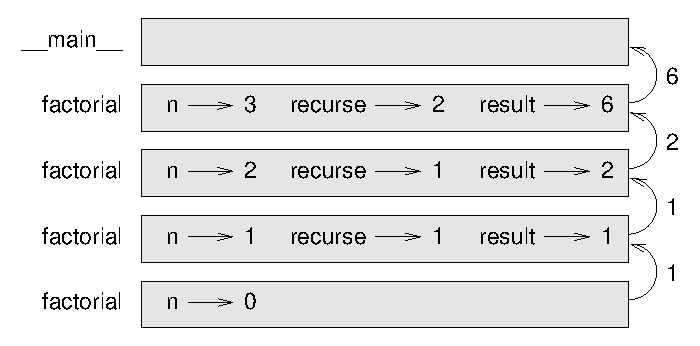
\includegraphics{figs/stack3.eps}}
\afterfig
\vspace{0.1in}

如图所示,返回值通过栈向上传递。在每一帧中,返回值是{\tt result}的值,即 {\tt n} 和 {\tt recurse}的乘积。

\index{帧}

在最后一帧中,局部变量 {\tt recurse} 和 {\tt result} 并不存在,因为该分支并没有创建它们。


\section{信心的飞跃}
\index{递归}
\index{信心的飞跃}

按照程序执行流程是阅读程序的一个方法,但这么做很容易走入迷宫。这里给出另一个方法,我称之为“信心的飞跃”。当你遇到一个函数调用,你{\em 假设}函数执行无误,并返回正确的结果,而不是追溯程序执行流程。

事实上,当你调用内建函数时,你已经体验过信心的飞跃。当你调用 {\tt math.cos} 和 {\tt math.exp}时,你并不检查这些函数的主体。你仅仅假设它们是由优秀的程序员编写的,可以正常的工作。

这同样适用于你自己写的函数。例如,在章节~\ref{布尔}中,我们编写了一个叫做\verb"is_divisible"的函数,判断一个数是否可以被另一个数整除。一旦我们通过检查测试函数确信它可以正常工作,我们可以直接调用该函数,而不用再去查看函数主体。

\index{测试!信心的飞跃}

以上思想同样适用于递归程序。当你遇到递归调用,你应该假设递归调用工作正常(并返回正确结果),而不是跟着程序执行流程。你可以这么问你自己,“假设我可以得到$n-1$的阶乘,我应该怎么计算$n$的阶乘?”很明显,通过乘以$n$就可以了。

当然,假设程序工作正常,而事实上你还没有完成这个函数,这里有一些诡异,但这就是为什么称之为信心的飞跃!


\section{另一个例子}
\label{另一个例子}

\index{斐波纳契函数}
\index{函数!斐波纳契}

除了 {\tt 阶乘}外,最常见的递归定义的数学函数是 {\tt 斐波纳契}函数,其定义如下:\footnote{参见 \url{wikipedia.org/wiki/Fibonacci_number}。}:

\vspace{-0.25in}
\begin{eqnarray*}
&& \mathrm{fibonacci}(0) = 0 \\
&& \mathrm{fibonacci}(1) = 1 \\
&& \mathrm{fibonacci}(n) = \mathrm{fibonacci}(n-1) + \mathrm{fibonacci}(n-2);
\end{eqnarray*}
%
翻译成Python为:

\beforeverb
\begin{verbatim}
def fibonacci (n):
    if n == 0:
        return 0
    elif  n == 1:
        return 1
    else:
        return fibonacci(n-1) + fibonacci(n-2)
\end{verbatim}
\afterverb
%
如果你试图跟随执行过程,即使很小的数$n$,你的脑袋也会爆炸。但是根据信心的飞跃,假设两个递归调用工作正确,就很容易看出通过将两者相加你将得到正确的结果。

\index{执行流程}


\section{类型检查}
\label{监护人}

\index{类型检查}
\index{错误检查}
\index{阶乘函数}

如果我们调用 {\tt factorial} 函数时提供的参数是1.5会怎么样?

\index{运行时错误}

\beforeverb
\begin{verbatim}
>>> factorial(1.5)
RuntimeError: Maximum recursion depth exceeded
\end{verbatim}
\afterverb
%
看起来这将会是一个无穷的递归。这事怎么发生的?递归函数有一个初始情况————当 {\tt n == 0}。但是如果 {\tt n} 不是一个整数,我们将 {\em 错过} 初始状态并不断的递归。

\index{无穷递归}
\index{递归!无穷}

在第一次递归调用中, {\tt n} 的值是0.5。在下一次调用时,它变为 -0.5。接着,它变得越来越小(更朝负方向),永远不会为0。

我们有两种选择。我们可以推广 {\tt factorial}函数使之可以工作在浮点数,或者我们可以让 {\tt factorial} 检查参数的数据类型。第一个方法可以参考gamma函数\footnote{参考 \url{wikipedia.org/wiki/Gamma_function}。},超出了本书的范围。让我们看看第二个方法。

\index{gamma函数}

我们可以使用内建函数 {\tt isinstance} 来验证参数的数据类型。同时我们可以确保参数的正的:

\index{isinstance函数}
\index{函数!isinstance}

\beforeverb
\begin{verbatim}
def factorial (n):
    if not isinstance(n, int):
        print 'Factorial is only defined for integers.'
        return None
    elif n < 0:
        print 'Factorial is only defined for positive integers.'
        return None
    elif n == 0:
        return 1
    else:
        return n * factorial(n-1)
\end{verbatim}
\afterverb
%
第一部分处理非整数;第二部分捕获负数。在这两种情况下程序将打印错误信息,并返回 {\tt None}表示有错误发生:

\beforeverb
\begin{verbatim}
>>> factorial('fred')
Factorial is only defined for integers.
None
>>> factorial(-2)
Factorial is only defined for positive integers.
None
\end{verbatim}
\afterverb
%
如果通过了两个检查,我们知道 $n$ 是一个正整数,可以保证递归会终止。

\index{守护人模式}
\index{模式!监护人}

这个程序展示了一个称为{\bf 监护人}的模式。前两个条件扮演了监护人的角色,防止错误的参数造成代码运行的错误。监护代码保证了程序的正确性。


\section{调试}
\label{factdebug}

\index{调试}

将大的程序拆成小的函数的过程给出了合理的调试测试点。如果一个函数工作不正常,有三种情况需要考虑:

\begin{itemize}

\item 函数得到的参数有误,即先决条件没有满足。

\item 函数本身有误,即后决条件没有满足。

\item 返回之有误,或者使用方式不正确。

\end{itemize}

为了排除第一种可能性,你可以在函数开始部分添加{\tt print}语句,打印参数值(数据类型)。或和你可以直接编写代码检查先决条件。

\index{先决条件}
\index{后决条件}

如果参数没有问题,在每条{\tt return}语句前添加{\tt print}语句,打印返回值。可能的话手工检查结果。试图使用容易检查的参数来调用函数(参见章节~\ref{增量开发})。

如果函数工作正常,检查函数调用,确保返回值被正确使用(或被使用!)。

\index{执行流程}

在函数开始和结尾添加打印语句可以使程序流程更加明显。例如,下面给出带打印语句的{\tt factorial}函数:

\beforeverb
\begin{verbatim}
def factorial(n):
    space = ' ' * (4 * n)
    print space, 'factorial', n
    if n == 0:
        print space, 'returning 1'
        return 1
    else:
        recurse = factorial(n-1)
        result = n * recurse
        print space, 'returning', result
        return result
\end{verbatim}
\afterverb
%
{\tt space}是空格的字符串,用来缩进输出结果。下面给出{\tt factorial(5)}的输出结果:

\beforeverb
\begin{verbatim}
                     factorial 5
                 factorial 4
             factorial 3
         factorial 2
     factorial 1
 factorial 0
 returning 1
     returning 1
         returning 2
             returning 6
                 returning 24
                     returning 120
\end{verbatim}
\afterverb
%
如果你不清楚程序执行的流程,这样的输出信息很有帮助。搭建脚手架会花费一些时间,但会帮助节省很多调试时间。


\section{术语}

\begin{description}

\item[临时变量:] 在复杂的计算过程中用来记录中间值的变量。
\index{临时变量}
\index{变量!临时}

\item[死区代码:] 程序中无法执行到的代码,通常因为出现在 {\tt return} 语句的后面。
\index{死区代码}

\item[{\tt None}:]  一个特殊的函数返回值,表明函数没有返回语句,或者返回语句没有参数。
\index{None特殊值}
\index{特殊值!None}

\item[增量开发:] 一种程序开发的方法,通过每次添加测试少量代码来避免程序的调试。
\index{增量开发}

\item[脚手架:] 在程序开发过程中使用的代码,并不出现在最终版本中。
\index{脚手架}

\item[守护人:] 使用条件语句检查错误并处理可能出错的情况的编程模式。
\index{守护人模式}
\index{模式!守护人}

\end{description}


\section{练习}

\begin{ex}
\index{栈图}

画下面程序的栈图。程序执行时会打印什么内容?

\beforeverb
\begin{verbatim}
def b(z):
    prod = a(z, z)
    print z, prod
    return prod

def a(x, y):
    x = x + 1
    return x * y

def c(x, y, z):
    sum = x + y + z
    pow = b(sum)**2
    return pow

x = 1
y = x + 1
print c(x, y+3, x+y)
\end{verbatim}
\afterverb

\end{ex}


\begin{ex}
\index{Ackerman函数}
\index{函数!ack}

Ackermann函数,$A(m, n)$,定义为\footnote{See \url{wikipedia.org/wiki/Ackermann_function}。}:

\begin{eqnarray}
A(m, n) = \begin{cases} 
              n+1 & \mbox{if } m = 0 \\ 
        A(m-1, 1) & \mbox{if } m > 0 \mbox{ and } n = 0 \\ 
A(m-1, A(m, n-1)) & \mbox{if } m > 0 \mbox{ and } n > 0.
\end{cases} 
\end{eqnarray}
%
编写一个 {\tt ack}的函数来计算 Ackerman's 公式。使用你的函数来计算 {\tt ack(3, 4)},结果应该是125。如果选择大的 {\tt m} 和 {\tt n}会发生什么?

\end{ex}


\begin{ex}
\label{回文}

\index{回文}

回文是一个从前往后和从后往前拼写相同的单词,如“noon”和“redivider”。从递归的角度来看,如果一个单词第一个字母和最后一个字母相同,且中间是回文的,那么这个单词是回文的。

下面的函数读取一个字符串作为参数,分别返回第一个、最后一个和中间的字母:

\beforeverb
\begin{verbatim}
def first(word):
    return word[0]

def last(word):
    return word[-1]

def middle(word):
    return word[1:-1]
\end{verbatim}
\afterverb
%
我们会在章节~\ref{strings}学习它们是如何工作的。

\begin{enumerate}

\item 在{\tt palindrome.py}文件中输入这些函数并测试。如果你输入两个字母,调用{\tt middle}会返回什么?一个字母呢?空字符串呢(使用\verb"''"输入,不包含任何字母)?

\item 编写函数\verb"is_palindrome",读取一个字符串作为参数,如果是回文则返回{\tt True},否则返回{\tt False}。你可以使用内建的{\tt len}函数来检查字符串的长度。

\end{enumerate}

\end{ex}

\begin{ex}
数$a$称为数$b$的幂,如果$a$可以被$b$整除,同时$a/b$是$b$的幂。编写函数\verb"is_power",读取{\tt a}和{\tt b}作为参数,如果{\tt a}是{\tt b}的幂则返回{\tt True}。
\end{ex}


\begin{ex}

\index{最大公约数(GCD)}
\index{GCD(最大公约数)}

最大公约数(GCD)是可以整除$a$和$b$最大的书\footnote{本练习基于Abelson and Sussman's {\em Structure and Interpretation of Computer Programs}的习题。}。

寻找两个数的GCD的一个方法是欧几里得算法,算法指出如果$r$是$a$除以$b$的余数,那么$gcd(a, b) = gcd(b, r)$。对于基本情况,我们考虑$gcd(a, 0) = a$。

\index{欧几里得算法}
\index{算法!欧几里得}

编写函数\verb"gcd" ,参数为{\tt a}和{\tt b},返回值为两者的最大公约数。如果你需要帮助,参考\url{wikipedia.org/wiki/Euclidean_algorithm}。

\end{ex}

